\section{Proposed Methods}
In order to complete the goals we have outlined, we have split the project into a few major sections. First and foremost is the simulation environments, which will help us debug and develop our algorithms. Second major goal is to plan the path of an inchworm from one place to another, a path planning algorithm will be developed and implemented. Finally,  a motion planning algorithm will be given the path created and simulate the robot walking the path.

\subsection{Simulation Environment}
Since the Covid-19 pandemic is preventing testing with physical hardware, a full physics simulator will be used to test the motion planning software that is designed and implemented. Simple simulators will also be developed to aid in the development of complicated path planning algorithms.

\begin{figure}[ht]
    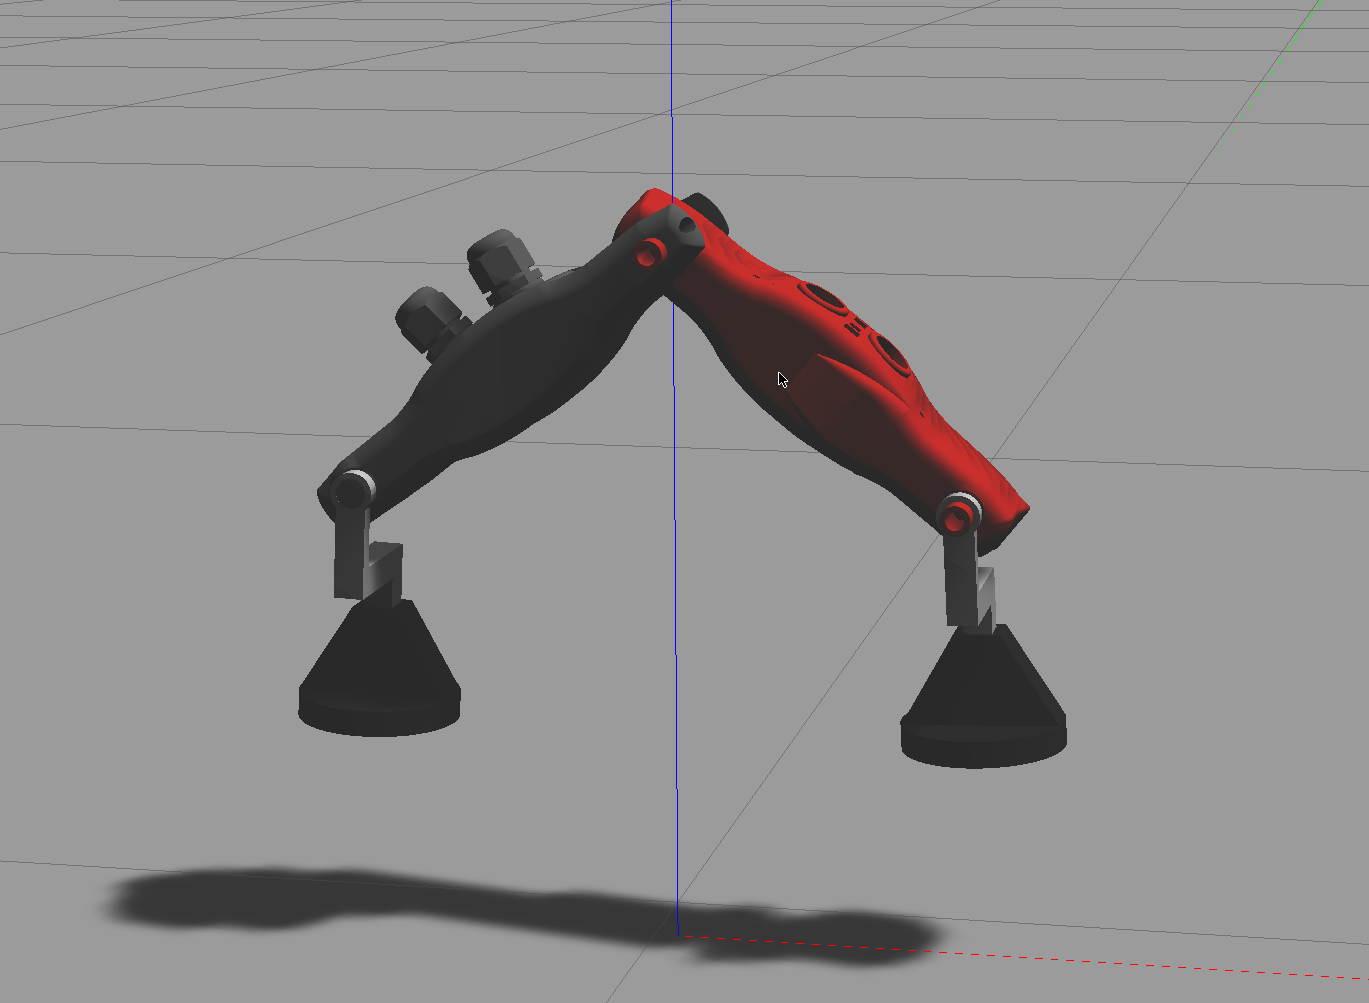
\includegraphics[width=\linewidth]{figures/GazeboSim.png}
    \caption{Inchworm modeled in Gazebo (simulator) \cite{PastMQP}}
    \label{fig:InchwormSim}
\end{figure} 

RVIZ will be the tool of choice to display and loosely simulate the path planning algorithms developed. Since physics is not considered, many of the variables that are not necessary for initial development of the path planning and footstep algorithms can be isolated and temporarily removed to simplify the software. These sudo-simulators can also be turned into visualizers to better understand what the system is doing when all of the algorithms are implemented and running together.

To test the robot in a virtual playground, a Gazebo simulator will be used with a playground and inchworm model. Since Gazebo is a full physics simulator, the inchworm model will need to include mass, inertia, and a semi-accurate model of the end effector. This includes a method to approximate the magnetic end effector of the inchworm. A Gazebo Vacuum Gripper Plugin will be used to achieve this \cite{GazeboVacuumGripper}\cite{MagnetFeetAnswers}, since the desired effect of a magnetic gripper is similar to a vacuum gripper, and developing a new plugin for Gazebo is out of the scope of this project. If we reach our expected goals, a model of the cube will be developed, which will include its own controller to simulate the connection between different cubes.

\subsection{Path Planning}
A path planning algorithm will be implemented to generate a path between the current position of the robot and the goal node, as determined by a higher-level system. The system should consider several robot conditions, including (but not limited to) inchworm step limitations, movement constraints, and collision avoidance \cite{CollisionAvoidance} (if the project progresses to a point where the inchworm is being tested in a cluttered environment). Several path planning algorithms are currently being considered, including A*, RTT*\cite{RT_RTT}, and RAGS (Risk Averse Graph Section). A relatively simple algorithm (A* or RTT*) will likely be implemented first, since initially the inchworm will be tested on a perfectly level and empty playground. If time allows, RAGS \cite{RAGS} may be implemented and compared to other algorithms, especially if the project leads to more advanced 3D graphs and maps.

The map is very important to a successful path planning algorithm. This project will initially use a simple 2 dimensional map (stored as a graph) to simplify the initial implementation of the path planning algorithm developed. If the climbing reach goal [insert ref to goal] is attempted, the map will need to consider a 3 dimensional environment. The first solution to be tested will be a “2.5” dimensional map, where the height will be added as a 3rd parameter. This may work for situations where the inchworm will only use the upward-facing face of the blocks in a structure. For situations where more advanced climbing is required, a fully 3-dimensional map will be required.

A map also needs to be generated given a playground. Perception is beyond the scope of this project, so the map will be generated based on a list of building blocks and their positions maintained by Gazebo. Initially for the 2 dimensional map, occupancy grids will be used as the map data structure, and blocks will be considered obstacles to be avoided by the robot. If the project leads to a 3 dimensional map, octrees are planned to be used as the map’s underlying data structure. One limitation that may cause issues during development is definition of what is graspable and what is not. To solve this, the occupancy grid may also contain information on the graspability of the position. This information will then be relayed back to the main path planner to be considered as a heuristic.

\subsection{Motion Planning}
The second major part of this project is the motion planning of the inchworm itself. While the path planning algorithm is in charge of determining an achievable path for the inchworm, the motion planning algorithms implemented will be in charge of actually executing that path. This major task can further be split into three major sections: inchworm kinematics, movement gaits, and footstep planning.

The 5 degree-of-freedom inchworm kinematics will be kept relatively simple, and dynamics will be automatically considered by a smart joint controller built into ROS and Gazebo \cite{ROSControl}. This is meant to simplify the development of the project, since dynamics of the robot is beyond the scope of this project. The overall kinematics of the inchworm will be similar to a robot arm, since the robot will have a stationary base during the movement gaits. However, two different kinematic controllers will need to be developed, depending what side of the inchworm is grounded \cite{PlanarInchWormDesign}.

\begin{figure}[ht]
    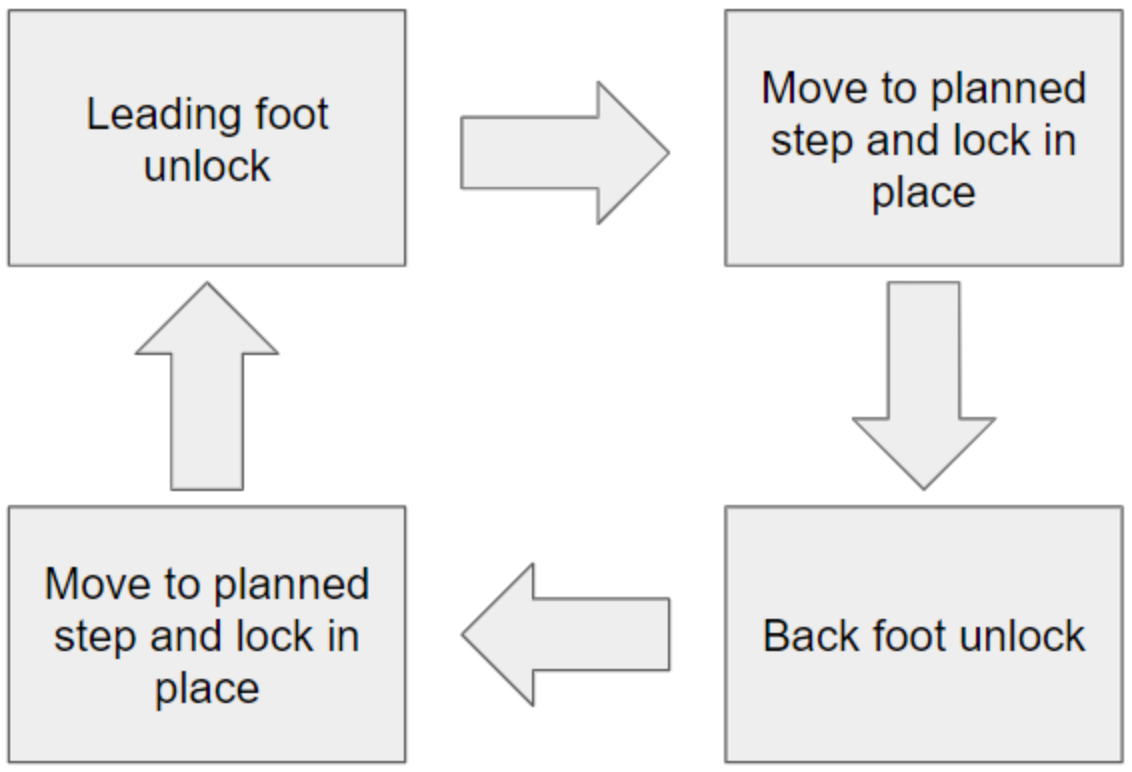
\includegraphics[width=\linewidth]{figures/GaitFlowChart.png}
    \caption{Our movement gait state machine flowchart}
    \label{fig:GaitFlowChart}
\end{figure} 

The movement gaits include the general walking gait and the climbing gait. Ideally, both gaits will be combined into one main gait which can climb and walk around a playground. The gait itself will essentially be a large state machine (see \autoref{fig:GaitFlowChart}). Initially, the robot is assumed to be in a position where both end effectors are locked into the playground. The leading foot will then be unlocked and moved to the next footstep position (as generated by the footstep planner). Then the leading foot will be placed in the correct position and locked down. Finally the back foot will unlock and move to its designated footstep position, and lock down. The cycle will loop back to the beginning until the inchworm reaches its final footstep position \cite{InchwormLocomotion} \cite{GaitGeneration} \cite{LeggedRobotsNavPlanning}.

\begin{figure}[ht]
    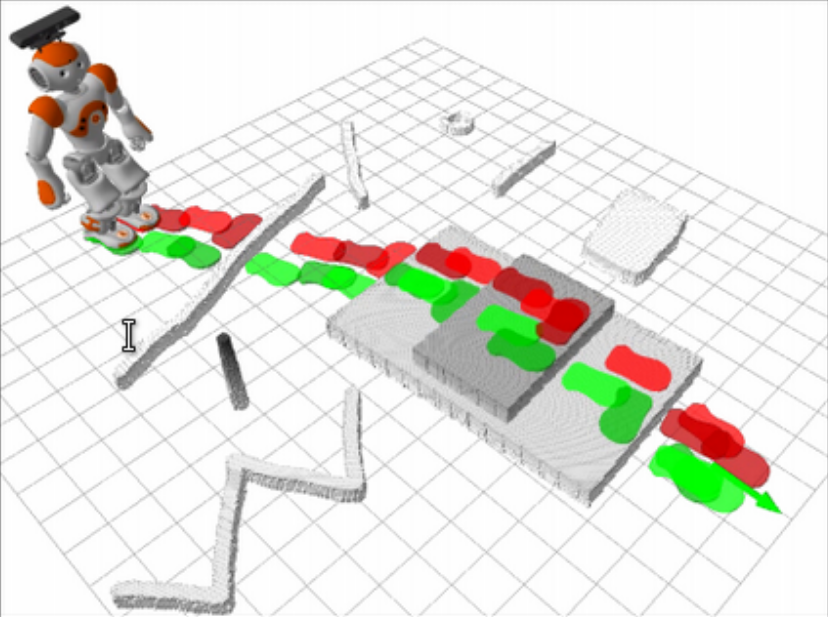
\includegraphics[width=\linewidth]{figures/FootStepPlanner.png}
    \caption{An graphical example of a search-based footstep planning using a 2-legged humanoid robot \cite{SearchFootstepPlanner}}
    \label{fig:FootstepPlannerExample}
\end{figure} 

The final part of the motion planner will be the footstep planner. Inspiration will be taken from bipeds and quadrupeds \cite{LeggedRobotsNavPlanning}, as many footstep planners exist for those types of robots. There are two options for footstep planners for the inchworm. A preemptive footstep planner generates all possible footsteps from any one location recursively, and places them in a graph. Then it can use a graph search (like A*, WA*, ARA*, RAGS, etc) to find the optimal footsteps throughout the path \cite{SearchFootstepPlanner}. This option is the simplest and will likely be the one implemented for this project. However, a more comprehensive and complete system is a dynamically generating real-time footstep planner. Such an algorithm can choose the best footsteps as the inchworm is moving, given real-time map data and information, by implementing modified versions of existing model predictive control algorithms (such as SLQ - Sequential Linear Quadratic - controllers) with different heuristics \cite{MotionPlanningInchworm} \cite{ModelPredictiveControl}. While this algorithm can lead to a much more comprehensive and complete footstep planner in dynamic environments, it is also relatively over-complicated for the static playground that we are assuming to test the inchworm in simulation.